\chapter{Asking Bugatti Owners How They Got Rich}

These notes follow Lecture 49 of the School of Hard Knocks interview series, presented here as a companion chapter curated by LazyingArt LLC. The lecture is built with a strict rhythm: first spectacle, then number, then doctrine, and only later mechanism. We move from a Bugatti and a handful of arresting claims to a more serious inquiry into capital, client concentration, trust, seller finance, delegation, and the human structure required to sustain ambition.

\section{Cold Open: Bugatti and the Numerical Shock}

We begin not with explanation but with a luxury object and a demand for compression. A Bugatti is presented, and the lecture immediately converts that sight into a string of quantities. We should be careful here. The cold open is a montage, not yet a single model. Its job is to convince us that the later search for mechanism is worth undertaking.

\begin{align}
V_{\text{Deepwater}}&=\$28\,\text{million},\\
R_{\text{day}}&=\$80\,\text{million},\\
Y_{\text{after-tax}}&=\$15\,\text{million},\\
T_{\text{federal}}&=0.
\end{align}

Each of these belongs to a distinct local claim. One is a legal case outcome, one is a day of business scale, one is a personal after-tax year, and one is a federal-tax claim tied later to real-estate law. The lecture deliberately places them side by side before it tells us how they were generated.

It is useful to freeze the opening as a simple value strip. This is not a proof; it is the lecture's promise.

\begin{figure}
\centering
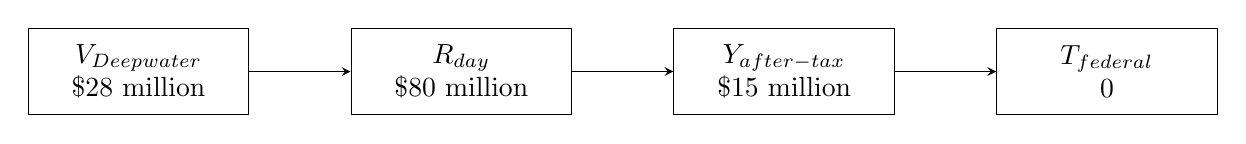
\begin{tikzpicture}[>=stealth]
\node[draw, rectangle, align=center, minimum width=2.8cm, minimum height=1.1cm] (a) at (0,0) {$V_{\text{Deepwater}}$\\$\$28$ million};
\node[draw, rectangle, align=center, minimum width=2.8cm, minimum height=1.1cm] (b) at (4.1,0) {$R_{\text{day}}$\\$\$80$ million};
\node[draw, rectangle, align=center, minimum width=2.8cm, minimum height=1.1cm] (c) at (8.2,0) {$Y_{\text{after-tax}}$\\$\$15$ million};
\node[draw, rectangle, align=center, minimum width=2.8cm, minimum height=1.1cm] (d) at (12.3,0) {$T_{\text{federal}}$\\$0$};
\draw[->] (a) -- (b);
\draw[->] (b) -- (c);
\draw[->] (c) -- (d);
\end{tikzpicture}
\end{figure}

The pedagogical effect is simple and powerful. Before we are told what to think, we are made to ask what sort of business life could plausibly produce these numbers.

\section{Scottsdale Reset and the Denial of Capital}

After the teaser the host resets the scene in Scottsdale and states the governing promise of the lecture: he will ask wealthy operators for the playbook that built their money and for the blueprint that a viewer might imitate. The first full case is a commercial-real-estate operator, and the first true obstacle raised by the lecture is the standard claim that one needs a great deal of capital just to begin.

\subsection{Question \& Answer}

\paragraph{Question.} Do we really need a great deal of capital to get started?

\paragraph{Answer.} The answer given in the interview is a hard rejection of that folk theorem, or at least a rejection of its usual form. The speaker substitutes for initial capital three other inputs: judgment, hard work, and the willingness to attack when circumstances collapse. We should not overstate the claim into a theorem that cash never matters. What the lecture is doing is more specific. It is shifting attention away from passive complaint and toward operating capacity.

The interview immediately tests this rhetoric against a number. The speaker's best year is stated as personal income, not company turnover:

\begin{equation}
Y_{\text{self,max}}=\$3.75\,\text{million}.
\end{equation}

That distinction matters. In this section of the lecture the host keeps asking for the amount that ended in the operator's hands, not merely a gross number for the business. The chapter should preserve that emphasis.

The interview closes this first argumentative pass by moving from business posture to personal interiority. Confidence is described not as a mystical gift but as something that followed visible results. Faith, by contrast, arrives later and is described as having become important even if it was not the first support.

\section{Land, Specialization, and a Small Client Base}

The lecture now narrows. The same operator explains why real estate became his vehicle. The answer is not a grand theory in advance. It is contingency disciplined by fit. He had expected to go toward stocks, interviewed at Grub \& Ellis, found that land was the available opening, and discovered that a family background in ranching and farming gave him a way into that niche because he understood farmers.

This is a recurring lesson in the interview corpus. We do not begin from abstract industry prestige. We begin from a place where prior knowledge lets us read a market more concretely than other people can.

The most striking claim in this portion is not the industry label but the client structure:

\begin{equation}
N_{\text{core clients}}\approx 2\text{ to }3,
\qquad
R_{\text{total}}=\sum_{i=1}^{N_{\text{core clients}}} R_i.
\end{equation}

The second formula is merely a useful schematic. The lecture does not give a ledger. But it does give the central idea: in certain high-ticket businesses, a few repeating relationships can dominate the sum.

\subsection{Question \& Answer}

\paragraph{Question.} Why can a very small client base be enough in a high-ticket business?

\paragraph{Answer.} Because the relevant variable is not the number of names in a database but the size, frequency, and durability of the transactions attached to a few trusted relationships. The operator's doctrine is not that every business should ignore breadth. It is that in his line of work, redundancy and friendship with a very small number of serious clients are more valuable than serving a thousand marginal accounts.

The lecture then hardens this into doctrine. Business school is treated skeptically, not because theory is worthless, but because the operator believes that many professors are distant from real risk. The local maxim that survives the section is even starker: never quit. That is not a mathematical statement. It is a separator the speaker treats as decisive.

\section{The Car Business: Iteration, Truth, and One-Day Scale}

A sponsor interruption breaks the motion. When the lecture resumes, it resumes correctly: another Bugatti, another number, and another mini-case. But the thematic center is now different. We move from real estate and concentrated clients to the car business, temperament, experimentation, and the production of trust.

The speaker again offers the lecture one of its defining quantities:

\begin{equation}
R_{\text{day}}=\$80\,\text{million}.
\end{equation}

We are not told whether this is gross sales, transaction volume, or another business measure, so we should keep the quantity speaker-attributed and narrow. The lecture's real work begins only after the number lands. The host asks about school. The answer is that poor performance in school, retrospectively interpreted through ADD, became a commercial advantage because it yielded creativity, energy, and vision, provided that calmer and more focused operators were placed nearby.

The lecture's non-numerical state diagram appears here with unusual clarity:

\begin{equation}
\text{iteration}\to\text{failure}\to\text{learning}\to\text{improvement}.
\end{equation}

This is drawn from the contrast between repeated rocket launches that fail and teach, and long waits for a supposedly perfect launch. The point is not aerospace. The point is business posture: a market teaches those who are willing to put incomplete attempts into the world.

\subsection{Question \& Answer}

\paragraph{Question.} What creates trust in a high-ticket sales business?

\paragraph{Answer.} The answer given here is exceptionally plain: tell the truth, under-promise, over-deliver, and keep your word. The lecture then strengthens that doctrine with an empirical consequence. A customer in Dubai tells the seller that the cars arrive better than described, not worse, and therefore he is comfortable buying sight unseen. Trust, in other words, reduces verification cost.

This is the most useful way to read the famous handshake doctrine in the interview. It is not nostalgia for a vanished world. It is an argument that reliable description and honored commitments lower friction and increase repeat business.

The section ends by widening that trust structure into private life. The choice of spouse is described not romantically but strategically: if the person nearest to us fights the work, friction rises; if the person nearest to us joins the work, the whole enterprise becomes more stable.

\section{Out-of-the-Box Improvement and Honest Negotiation}

The next speaker shifts the lecture away from asset class and toward process. His language is eccentric but the underlying structure is legible. He does not say that he thinks inside a box and optimizes it a little. He says he thinks out of the box, even that he ``builds triangles.'' We should not literalize the geometry. The point is refusal of the given frame.

The origin story is severe. In 1970 he is sleeping in his car and asking for a better way. At McDonald's he sees a workflow with twelve people and starts altering small physical details: spatulas, bun placement, movement through the line. The lecture wants us to see continuity between these tiny redesigns and later large commercial outcomes, including the Deepwater Horizon case that he says generated \$28 million.

\subsection{Question \& Answer}

\paragraph{Question.} How does constant process improvement become a wealth engine?

\paragraph{Answer.} Because each local friction point can be treated as an opportunity for redesign, and a redesign repeated across enough transactions accumulates into real value. The lecture does not give a formal productivity equation. What it gives us is the more primitive operator's instinct: when a process feels awkward, change the geometry of the process.

The negotiation doctrine in this section is brutally compressed: ``100\% honesty, period.'' We should preserve the honesty and discard the rhetorical violence that accompanies it. The business content is simple. Deals close, and stay closed, when speech and reality line up.

The same structure appears again when the host asks about poverty escape. The answer is not elegant. It is sobriety, prayer, persistence, and the repeated question: what can I provide that other people do not? The lecture is consistent on this point. Wealth does not emerge merely from desiring more money. It emerges from seeing overlooked improvements and attaching them to a market.

\section{Pace Morby: Tax, Seller Finance, and Cash Flow}

Now the lecture becomes more explicit and almost ledger-like. Pace Morby is introduced as a nine-figure real-estate entrepreneur, and the host begins asking the kinds of questions that finally produce a mathematical payload: why real estate, how much money, why no federal income tax, how that can be legal, and how a property can be acquired without a bank, without credit, and without cash out of pocket.

The first bundle of numerical data is as follows:

\begin{align}
t_{\text{real estate}}&=12\ \text{years},
&
t_{\text{construction prior}}&=10\ \text{years},\\
Y_{\text{after-tax}}&=\$15\,\text{million},
&
R_{\text{company}}&\approx \$115\,\text{million}\ \text{per year},\\
P_{\text{portfolio}}&\approx \$500\,\text{million}.&
\end{align}

The speaker also makes the sharp tax claim that drives the rest of the section:

\begin{align}
Y_{\text{after-tax}}&=Y_{\text{pre-tax}}-T_{\text{federal}}-T_{\text{other}},\\
T_{\text{federal}}&=0,
\qquad
\Delta t_{\text{no federal tax}}=7\ \text{years}.
\end{align}

\begin{remark}
The lecture's claim is not that all taxation disappears. Pace explicitly says that property taxes and employment taxes remain. The strong claim is narrower: federal income tax has been reduced to zero through real-estate treatment in the tax code.
\end{remark}

The public-policy comparison that accompanies this argument is also numerical:

\begin{equation}
C_{\text{gov,unit}}\approx \$600{,}000,
\qquad
C_{\text{private,unit}}\approx \$75{,}000,
\qquad
\frac{C_{\text{gov,unit}}}{C_{\text{private,unit}}}\approx 8.
\end{equation}

We should keep this as a speaker-attributed comparison, not as a fully specified cost model. The lecture gives the ratio, not the construction ledger.

\subsection{Question \& Answer}

\paragraph{Question.} How can real estate produce large after-tax cash flow with no bank, no credit, and no cash out of pocket?

\paragraph{Answer.} The lecture's mechanism is seller finance. The steps are short and surprisingly clean.

\begin{enumerate}
\item A long-time owner wants to retire and prefers a monthly check.
\item A cash sale would create an immediate capital-gains event for the seller.
\item Seller finance converts the seller into the lender.
\item Tenant rent funds the buyer's payments and operating costs.
\end{enumerate}

For compactness we may summarize the buyer's entry conditions as

\begin{equation}
L_{\text{bank}}=0,
\qquad
X_{\text{credit}}=0,
\qquad
K_{\text{out}}=0.
\end{equation}

Again, this is editorial shorthand, not the speaker's own notation. It is a way of freezing the claim the lecture is making.

The mechanism can be drawn as a simple flow.

\begin{figure}
\centering
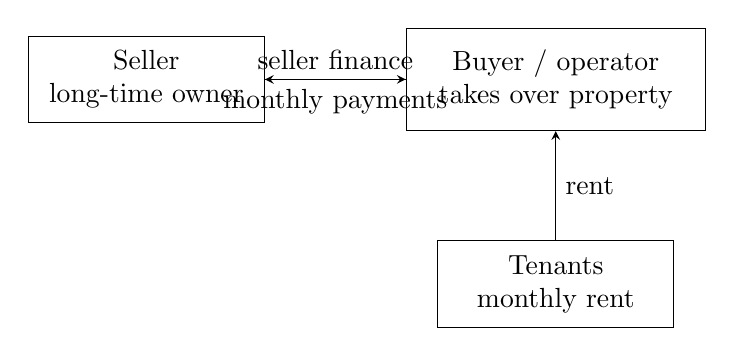
\begin{tikzpicture}[>=stealth]
\node[draw, rectangle, align=center, minimum width=3.0cm, minimum height=1.1cm] (seller) at (0,0) {Seller\\long-time owner};
\node[draw, rectangle, align=center, minimum width=3.8cm, minimum height=1.3cm] (buyer) at (5.2,0) {Buyer / operator\\takes over property};
\node[draw, rectangle, align=center, minimum width=3.0cm, minimum height=1.1cm] (tenants) at (5.2,-2.6) {Tenants\\monthly rent};
\draw[->] (seller) -- node[above]{seller finance} (buyer);
\draw[->] (buyer) -- node[below]{monthly payments} (seller);
\draw[->] (tenants) -- node[right]{rent} (buyer);
\end{tikzpicture}
\end{figure}

\paragraph{Worked example.} The lecture supplies one concrete property example, and this is the chapter's clearest explicit calculation. Taking the numbers at face value, we write

\begin{align}
CF_{\text{net}}
&=
R_{\text{tenants}}
-
P_{\text{seller}}
-
C_{\text{tax}}
-
C_{\text{insurance}}
-
C_{\text{management}}
-
C_{\text{repairs}},\\
N_{\text{units}}&=160,
\qquad
R_{\text{gross,month}}\approx \$160{,}000,
\qquad
CF_{\text{net,month}}\approx \$53{,}000.
\end{align}

If we treat the gross monthly figure as tenant revenue, then the combined monthly outflow is approximately

\begin{align}
P_{\text{seller}}+C_{\text{tax}}+C_{\text{insurance}}+C_{\text{management}}+C_{\text{repairs}}
&\approx
R_{\text{gross,month}}-CF_{\text{net,month}}\\
&\approx
\$160{,}000-\$53{,}000\\
&\approx
\$107{,}000.
\end{align}

The lecture does not provide enough detail for a full pro forma, but it does permit one useful scale ratio:

\begin{equation}
\frac{CF_{\text{net,month}}}{R_{\text{gross,month}}}
\approx
\frac{53}{160}
\approx
0.331.
\end{equation}

That number should be used cautiously. It is not a theorem about multifamily real estate. It is only a ratio extracted from the example offered in the interview.

\section{Scale, Complementarity, and Permission}

After the most technical section, the lecture returns to the human architecture of scale. First comes delegation. Then hiring. Then complementarity in partnership. The speaker's rule is blunt: pay high-quality people, and pair with someone whose skills oppose and complete our own.

A useful compression of this doctrine is

\begin{equation}
Q_{\text{scale}}
\approx
f(\text{delegation},\ \text{high-quality hires},\ \text{complementary partners}).
\end{equation}

This is not offered by the lecture as a formal model. It is a disciplined shorthand for what the speaker says in prose. One person attracts, teaches, and stands in public. Another runs payroll, books, management, and operational stability. The enterprise grows not by heroic unity of personality but by structured difference.

\subsection{Question \& Answer}

\paragraph{Question.} What kind of relationships make large-scale ambition durable?

\paragraph{Answer.} The lecture gives three answers at once. First, opposite-skill partners who complete a deficiency rather than mirror a strength. Second, friends and collaborators who already believe in the vision, rather than skeptics who must be persuaded endlessly. Third, a community that grants permission to grow. The lecture is explicit that many people close to us do not grant that permission, even when they mean well.

This section then turns sharply downward before it rises. Pace describes the suicide of his brother, a divorce, a family imprisonment, his own suicide note, and the phone call from his mother that interrupted the act. Only after this descent does the lecture return to arithmetic:

\begin{equation}
N_{\text{employees}}\approx 600,
\qquad
R_{\text{annual}}\approx \$100\,\text{million}.
\end{equation}

The order matters. The lecture does not say that numbers abolish suffering. It says something more severe: the same life can contain both catastrophic interior collapse and later large organizational scale. Community is therefore not a decorative moral afterthought. It is part of the mechanism by which ambition becomes survivable.

\section{Summary}

The lecture begins by spending surprise and ends by spending structure. First we are given spectacle: a Bugatti, \$28 million, \$80 million, \$15 million, zero federal income tax. Then we are given local doctrines: capital is not the only gate, a few clients may dominate an industry, truth compounds in sales, and small process improvements can accumulate into large value. Finally we are given mechanism: tax treatment, seller finance, operating cash flow, delegation, opposite-skill partnership, and community as permission. The result is not a universal theory of wealth. It is something narrower and more useful: a series of interview-derived cases in which money, method, and character are repeatedly braided together.